\section{Weitere Ergebnisse der adaptiven Irradianzschätzung} % (fold)
\label{sec:ergebnisse_adaptive_irradianzschaetzung}

	\begin{figure}[h]
		\begin{subfigure}[t]{0.33\textwidth}
			\center
			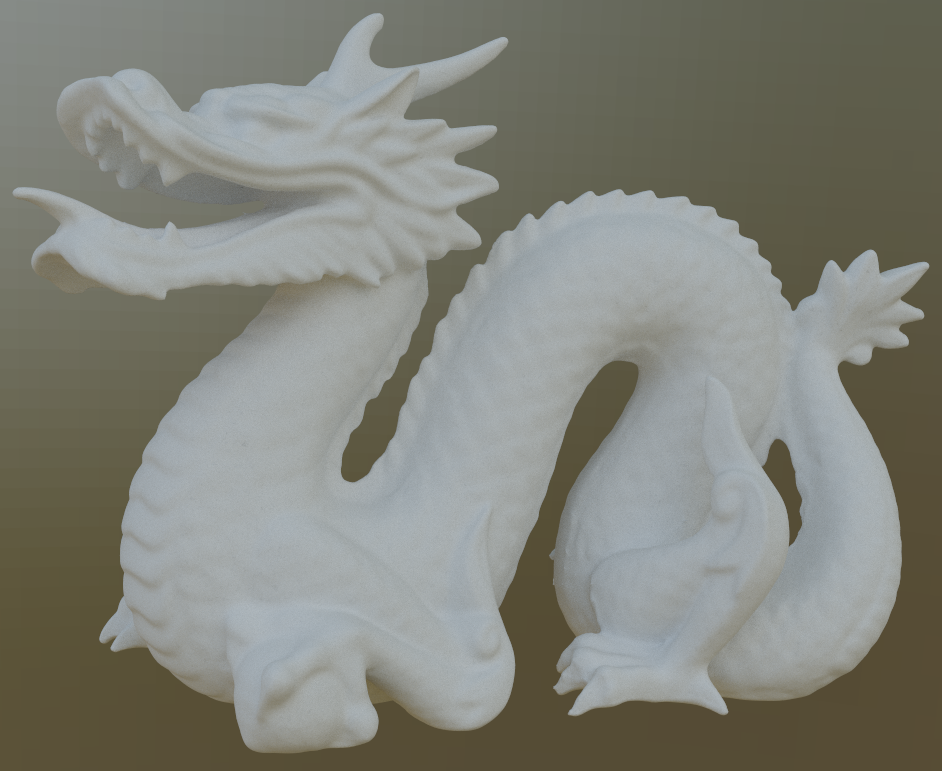
\includegraphics[width=0.95\textwidth]{pic/irr_est-ra-dragon-ref.png}
			\caption{Path Tracing}
			\label{subfig:irr-est-ra-dragon-ref}
		\end{subfigure}
		\begin{subfigure}[t]{0.33\textwidth}
			\center
			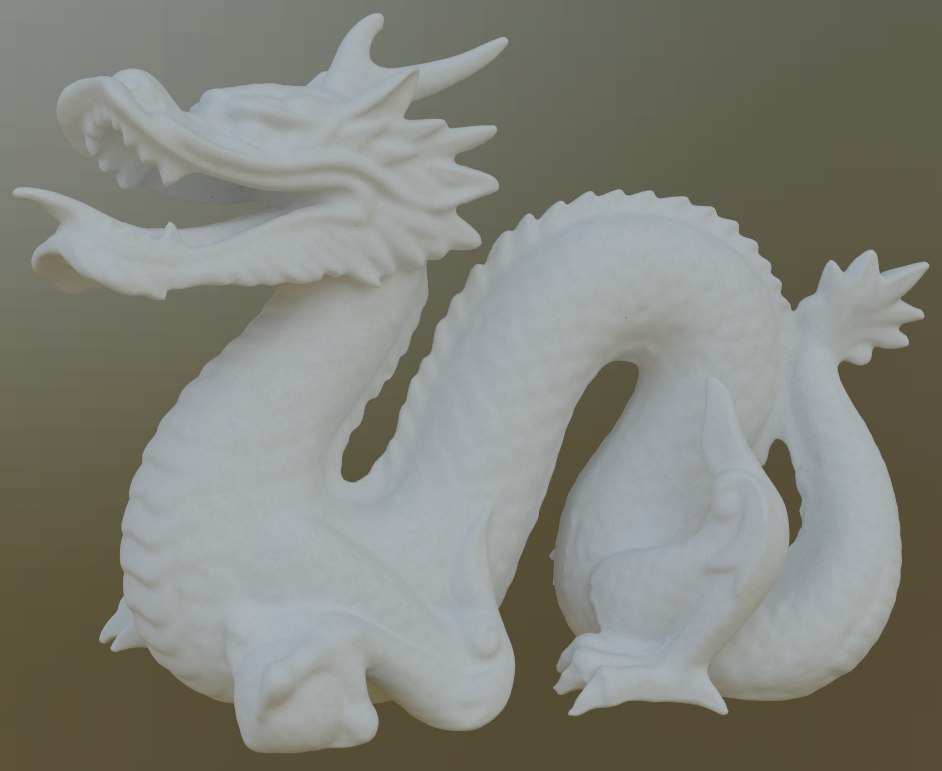
\includegraphics[width=0.95\textwidth]{pic/irr_est-ra-dragon-irr.png}
			\caption{Irradianz}
			\label{subfig:irr-est-ra-dragon-irr}
		\end{subfigure}
		% \medskip \\
		% \begin{subfigure}[t]{0.33\textwidth}
		% 	\center
		% 	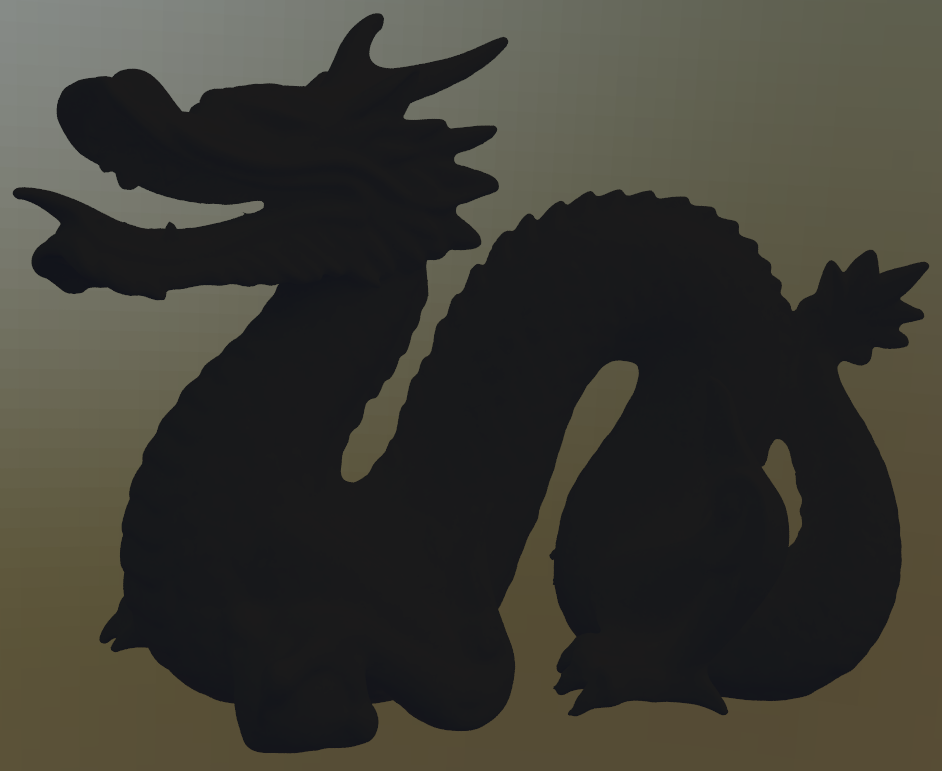
\includegraphics[width=0.95\textwidth]{pic/irr_est-ra-dragon-err.png}
		% 	\caption{Standardabweichung}
		% \end{subfigure}
		\begin{subfigure}[t]{0.33\textwidth}
			\center
			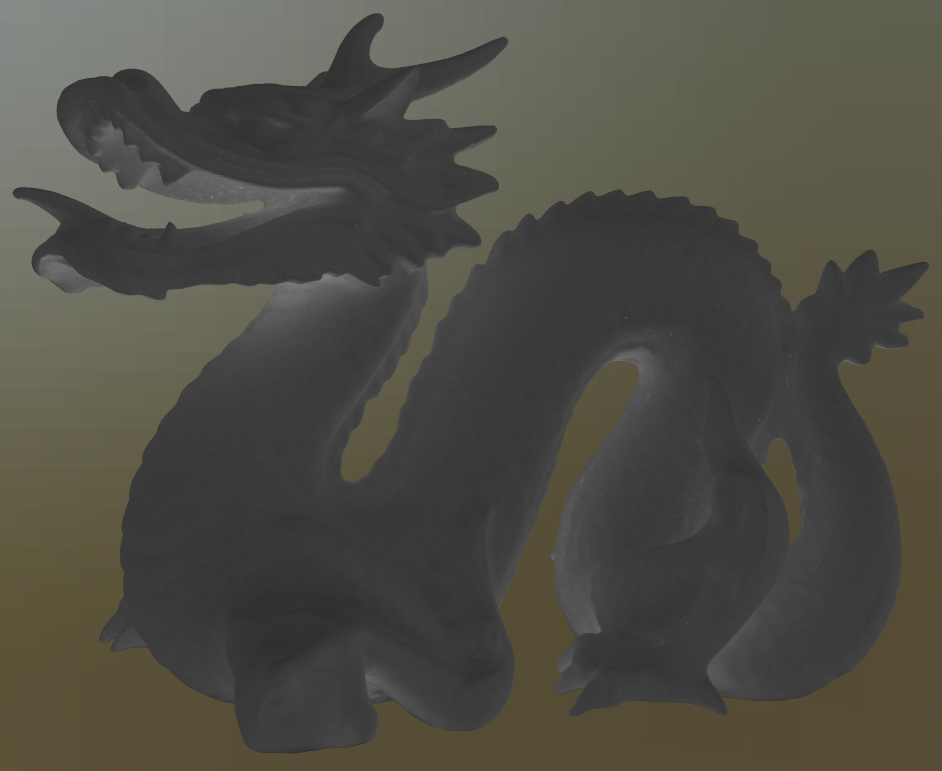
\includegraphics[width=0.95\textwidth]{pic/irr_est-ra-dragon-scount.png}
			\caption{Sampleanzahl}
			\label{subfig:irr-est-ra-dragon-scount}
		\end{subfigure}
		\caption[Erste adaptive Vertex-Irradiance-Map anhand der \enquote{Dragon}-Szene]{Die Bilder zeigen die \enquote{Dragon}-Szene mit einer schwach variierenden Umgebungsbeleuchtung. \ref{subfig:irr-est-ra-dragon-ref} ist das durch Path Tracing erzeugte Referenzbild. \ref{subfig:irr-est-ra-dragon-irr} zeigt die an den Eckpunkten adaptiv aufgenommenen Irradianzen mit linearer Interpolation. \ref{subfig:irr-est-ra-dragon-scount} stellt dabei die zugehörigen Sampleanzahlen dar. Hier bedeutet eine hellere Farbe eine höhere Sampleanzahl. Die Berechnungszeit betrug $253\unit{s}$ mit der maximalen Sampleanzahl $2^{16}$ und einem maximalen relativen Fehler von $3\unit{\%}$.

		Die ersten beiden dienen dem Vergleich der Korrektheit des Algorithmus. Das dritte Bild }
		\label{fig:irr-est-ra-dragon}
	\end{figure}

	\begin{figure}[h]
		\begin{subfigure}[t]{0.33\textwidth}
			\center
			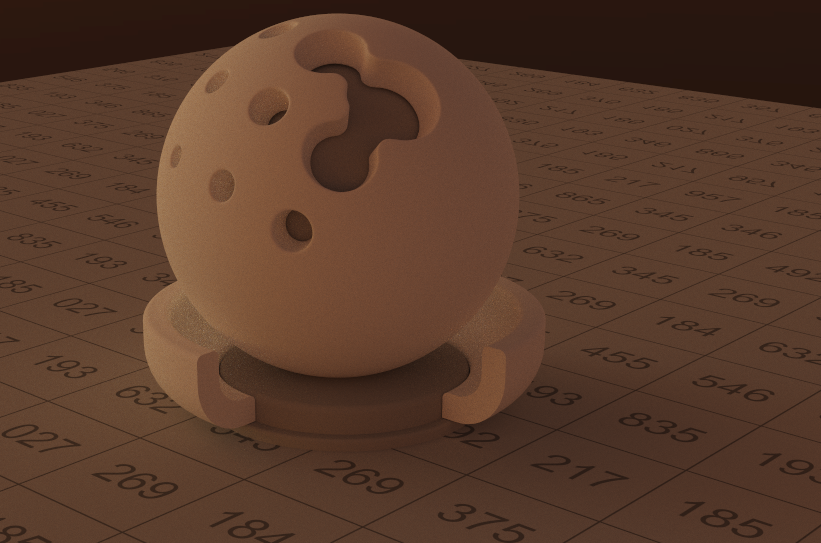
\includegraphics[width=0.95\textwidth]{pic/irr_est-ra-shaderball-ref.png}
			\caption{Path Tracing}
		\end{subfigure}
		\begin{subfigure}[t]{0.33\textwidth}
			\center
			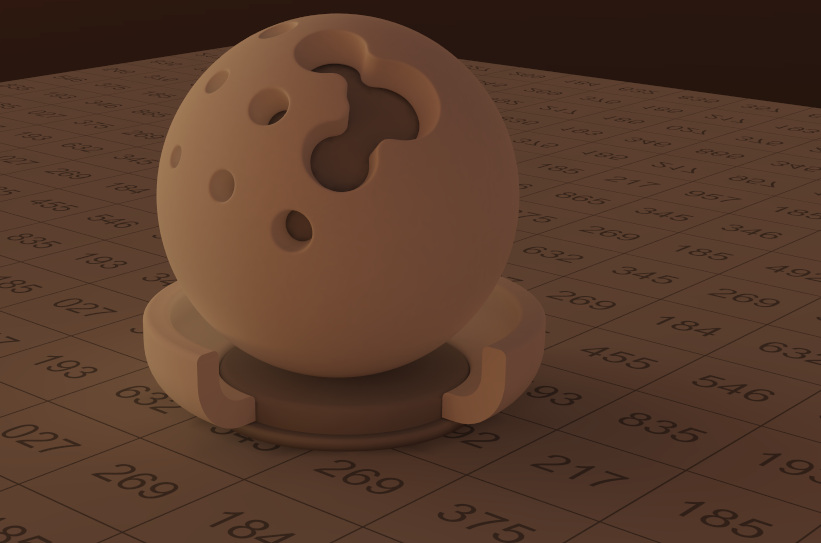
\includegraphics[width=0.95\textwidth]{pic/irr_est-ra-shaderball-irr.png}
			\caption{Irradianz}
		\end{subfigure}
		\begin{subfigure}[t]{0.33\textwidth}
			\center
			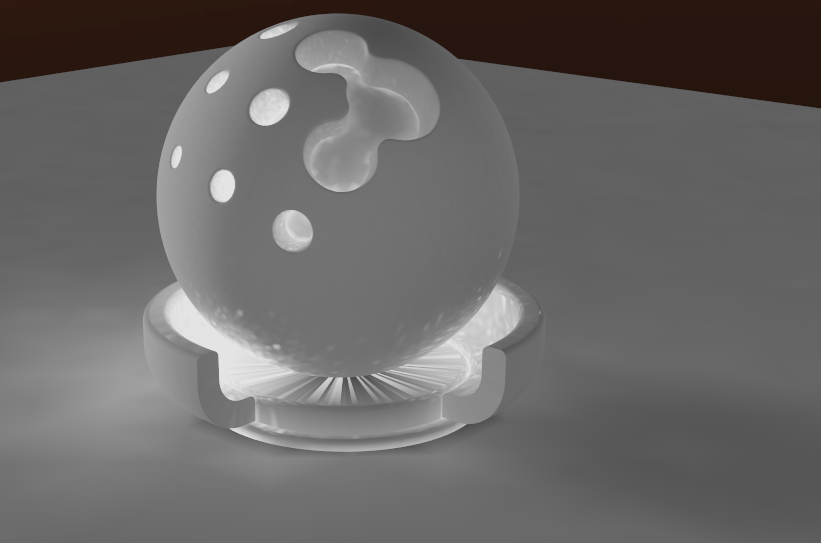
\includegraphics[width=0.95\textwidth]{pic/irr_est-ra-shaderball-scount.png}
			\caption{Sampleanzahl}
		\end{subfigure}
		\caption[Erste adaptive Vertex-Irradiance-Map anhand der \enquote{Shaderball}-Szene]{Die Bilder zeigen die \enquote{Shaderball}-Szene mit einer stark variierenden Umgebungsbeleuchtung analog zu Abbildung \ref{fig:irr-est-ra-dragon}. Die Berechnungszeit betrug $1170\unit{s}$ mit der maximalen Sampleanzahl $2^{18}$ und einem maximalen relativen Fehler von $1\unit{\%}$.}
		\label{fig:irr-est-ra-shaderball}
	\end{figure}

	\begin{figure}[h]
		\begin{subfigure}[t]{\textwidth}
			\center
			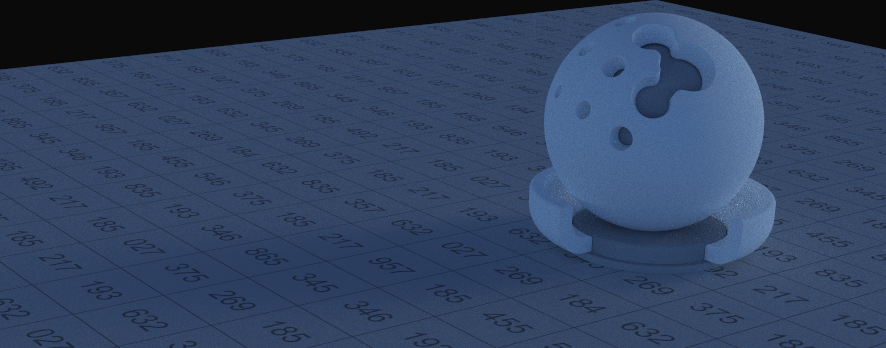
\includegraphics[width=0.95\textwidth]{pic/irr_est-ra-shaderball3-ref.png}
			\caption{Path Tracing}
		\end{subfigure}
		\medskip \\
		\begin{subfigure}[t]{\textwidth}
			\center
			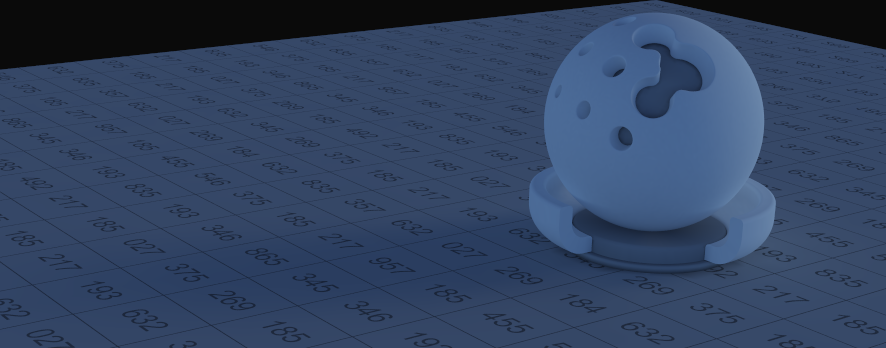
\includegraphics[width=0.95\textwidth]{pic/irr_est-ra-shaderball3-irr.png}
			\caption{Irradianz}
		\end{subfigure}
		\medskip \\
		\begin{subfigure}[t]{\textwidth}
			\center
			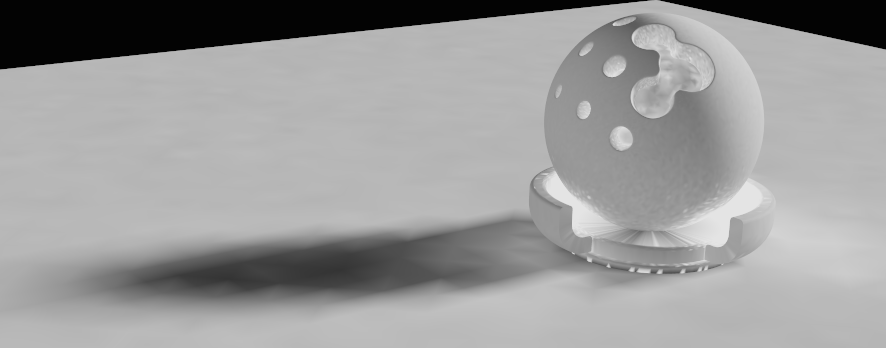
\includegraphics[width=0.95\textwidth]{pic/irr_est-ra-shaderball3-scount.png}
			\caption{Sampleanzahl}
		\end{subfigure}
		\caption[Dritte adaptive Vertex-Irradiance-Map anhand der \enquote{Shaderball}-Szene]{Die Bilder zeigen die \enquote{Shaderball}-Szene mit einer stark konzentrierten Umgebungsbeleuchtung analog zu Abbildung \ref{fig:irr-est-ra-dragon}. Die Berechnungszeit betrug $1090\unit{s}$ mit der maximalen Sampleanzahl $2^{18}$ und einem maximalen relativen Fehler von $1\unit{\%}$.}
		\label{fig:irr-est-ra-shaderball3}
	\end{figure}

	\begin{figure}[h]
		\begin{subfigure}[t]{\textwidth}
			\center
			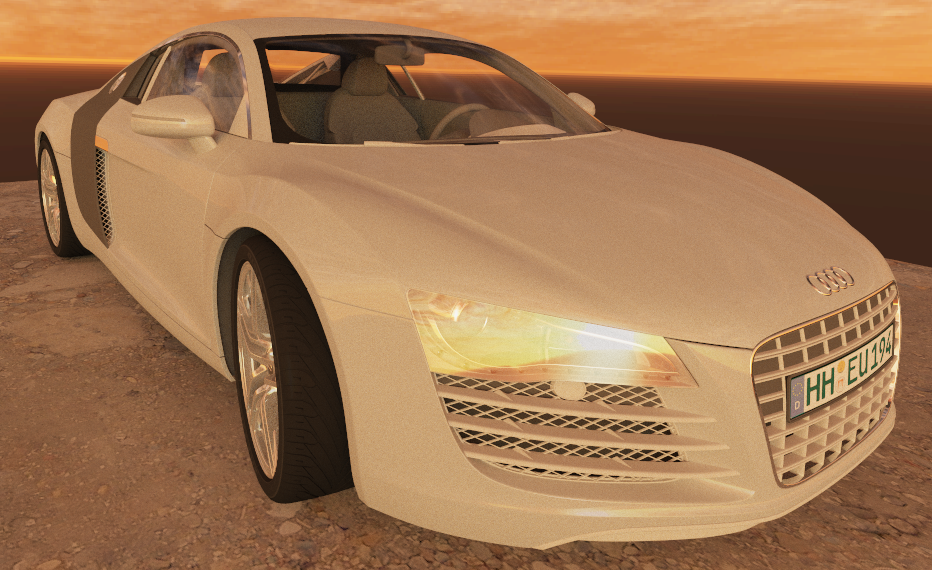
\includegraphics[width=0.8\textwidth]{pic/irr_est-ra-r8-ref.png}
			\caption{Path Tracing}
		\end{subfigure}
		\begin{subfigure}[t]{\textwidth}
			\center
			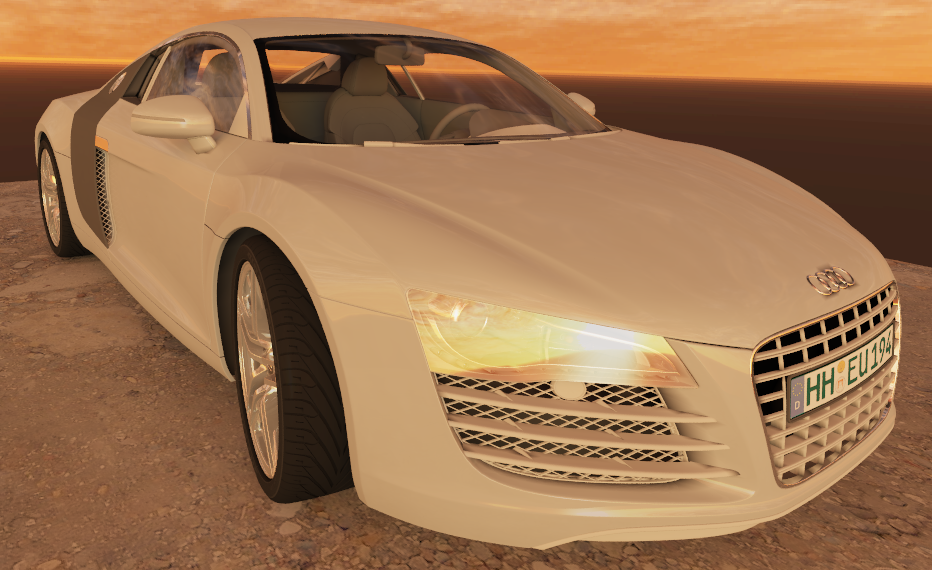
\includegraphics[width=0.8\textwidth]{pic/irr_est-ra-r8-irr.png}
			\caption{Irradianz}
		\end{subfigure}
		\begin{subfigure}[t]{\textwidth}
			\center
			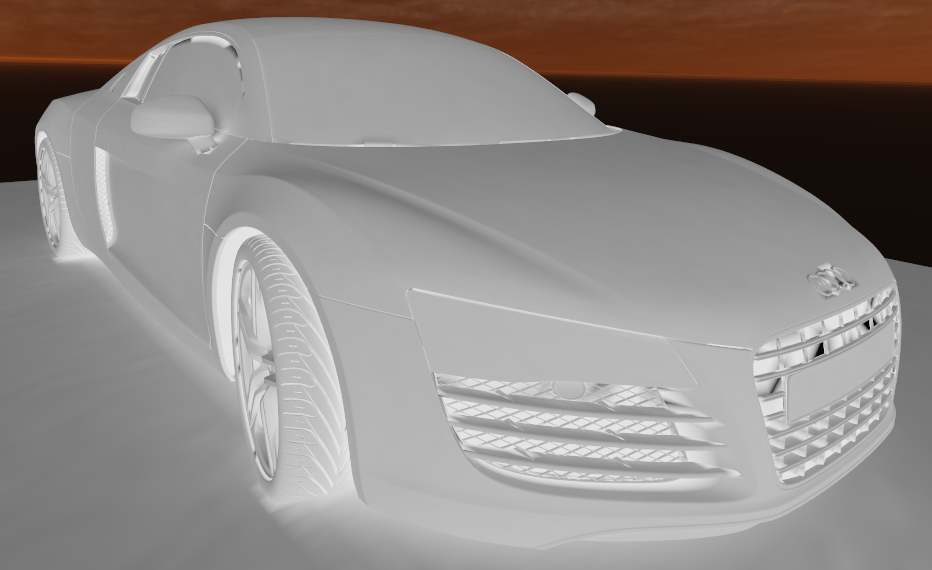
\includegraphics[width=0.8\textwidth]{pic/irr_est-ra-r8-scount.png}
			\caption{Sampleanzahl}
		\end{subfigure}
		\caption[Adaptive Vertex-Irradiance-Map anhand der \enquote{Audi R8}-Szene]{Die Bilder zeigen die \enquote{Audi R8}-Szene mit der \enquote{Sky 20}-Umgebungsbeleuchtung analog zu Abbildung \ref{fig:irr-est-ra-dragon}. Die Berechnungszeit betrug $17.8\unit{h}$ mit der maximalen Sampleanzahl $2^{18}$ und einem maximalen relativen Fehler von $1\unit{\%}$.}
		\label{fig:irr-est-ra-audi}
	\end{figure}

	\begin{figure}[h]
		\begin{subfigure}[t]{\textwidth}
			\center
			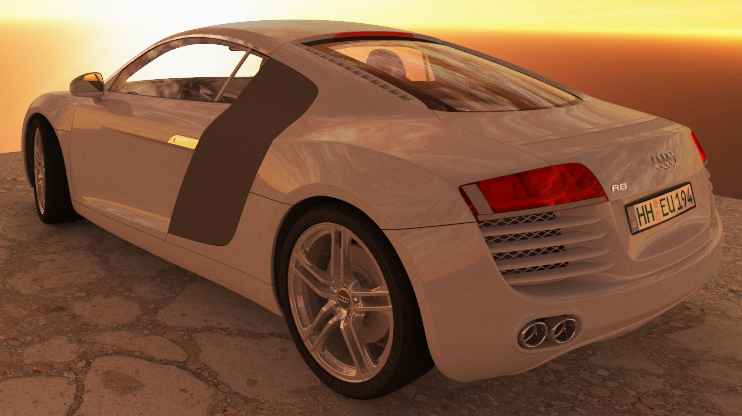
\includegraphics[width=0.85\textwidth]{pic/irr_est-ra-r8_2-ref.png}
			\caption{Path Tracing}
		\end{subfigure}
		\begin{subfigure}[t]{\textwidth}
			\center
			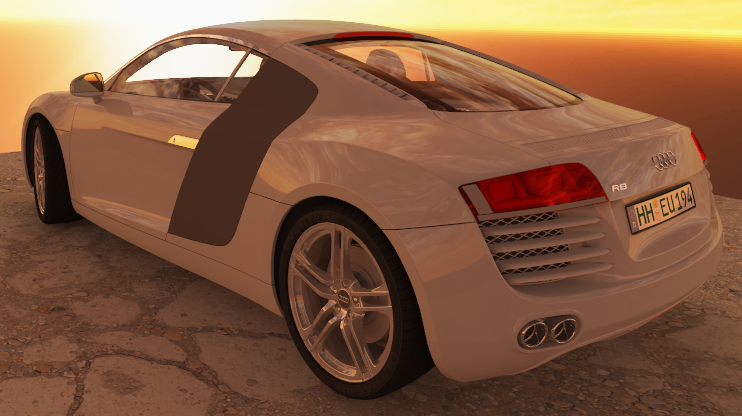
\includegraphics[width=0.85\textwidth]{pic/irr_est-ra-r8_2-irr.png}
			\caption{Irradianz}
		\end{subfigure}
		\begin{subfigure}[t]{\textwidth}
			\center
			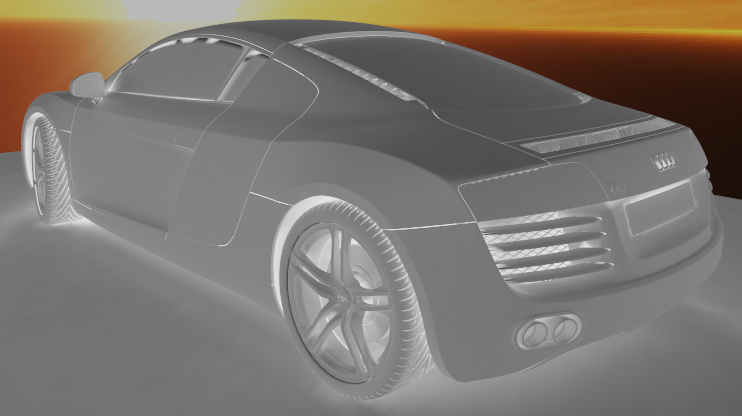
\includegraphics[width=0.85\textwidth]{pic/irr_est-ra-r8_2-scount.png}
			\caption{Sampleanzahl}
		\end{subfigure}
		\caption[Adaptive Vertex-Irradiance-Map anhand der \enquote{Audi R8}-Szene]{Die Bilder zeigen die \enquote{Audi R8}-Szene mit der \enquote{Sky 20}-Umgebungsbeleuchtung analog zu Abbildung \ref{fig:irr-est-ra-dragon}. Die Berechnungszeit betrug $17.8\unit{h}$ mit der maximalen Sampleanzahl $2^{18}$ und einem maximalen relativen Fehler von $1\unit{\%}$.}
		\label{fig:irr-est-ra-audi2}
	\end{figure}

% section weitere_ergebnisse_der_adaptiven_irradianzschätzung (end)